\usepackage{amsthm}

\newtheorem{theorem}{Theorem}[chapter]
\newtheorem{lemma}           [theorem] {Lemma}   
\newtheorem{folg}           [theorem] {Folgerung}   

\newtheorem{frage}       [theorem] {Frage}   
\newtheorem{question}       [theorem] {Question}   
\newtheorem{aufgabe}       [theorem] {Aufgabe}   
\newtheorem{exercise}       [theorem] {Exercise}  

\newtheorem{proposition}     [theorem] {Proposition}  
\newtheorem{satz}     [theorem] {Satz}  
\newtheorem{fact}{Fact}
\newtheorem{definition}      [theorem] {Definition} 

\theoremstyle{definition} 
\newtheorem{bemerkung}     [theorem] {Bemerkung}  
\newtheorem{beispiel}       [theorem] {Beispiel}  
\newtheorem{example}       [theorem] {Example}  
\newtheorem*{example*} {Example}  
\newtheorem{notation}       [theorem] {Notation}  
\newtheorem*{Faust}[theorem]{Rule of Thumb}
\newtheorem*{Boxx}[theorem]{Concept}
%\subsection*{Operations on sets}

We remember the important operations for sets:

\begin{itemize}
 \item $M_1 \cup M_2 := \{ x \mid x\in M_1 \vee x \in M_2 \}$ (union)
 \item $M_1 \cap M_2 := \{ x \mid x \in M_1 \wedge x \in M_2\}$ (intersection)
 \item $M_1 \setminus M_2 := \{ x \mid x \in M_1 \wedge x \not\in M_2 \}$ (set difference)
\end{itemize}

\begin{Definition}[Set compositions]
%\begin{figure}[htbp]
%   \begin{minipage}[c]{0.5\textwidth}
   The \emph{union} $M_1\cup M_2$ 
   is the new set that consists exactly
   of the objects that are elements of $M_1$ \textbf{or} $M_2$.
  
%   \end{minipage}
%   \begin{minipage}[c]{0.4\textwidth}
%   \flushright
%      \begin{tikzpicture}[scale=0.8] % M_1 vereinigt M_2
% \def\firstcircle{(0,0) circle (1.5cm)}
% \def\secondcircle{(0:2cm) circle (1.5cm)}
%     \draw[fill=black!15] \firstcircle node {\begin{footnotesize}$M_1$ \end{footnotesize}}
%                   \secondcircle node {\begin{footnotesize} $M_2$ \end{footnotesize}};
%     \node[anchor=south] at (current bounding box.north) {\begin{footnotesize} $M_1 \cup M_2$ \end{footnotesize}};
% \end{tikzpicture}
%   \end{minipage}
% %\end{figure}
% ~\\[4ex]
%\begin{figure}[htbp]
%  \begin{minipage}[c]{0.5\textwidth}
  The \emph{intersection} $M_1\cap M_2$ 
  is the new set
  whose elements 
  are the objects that are elements of $M_1$ \textbf{and} $M_2$.

%   \end{minipage}
%   \begin{minipage}[c]{0.4\textwidth}
%   \flushright  
%      \begin{tikzpicture}[scale=0.8] % M_1 geschnitten M_2
% \def\firstcircle{(0,0) circle (1.5cm)}
% \def\secondcircle{(0:2cm) circle (1.5cm)}
%     \begin{scope}
%         \clip \firstcircle;
%         \fill[fill=black!15] \secondcircle;
%     \end{scope}
%     \draw \firstcircle node {\begin{footnotesize} $M_1$ \end{footnotesize}};
%     \draw \secondcircle node {\begin{footnotesize} $M_2$ \end{footnotesize}};
%     \node[anchor=south] at (current bounding box.north) {\begin{footnotesize} $M_1 \cap M_2$ \end{footnotesize}};
% \end{tikzpicture}
%   \end{minipage}
%\end{figure}
% ~\\[4ex]
%\begin{figure}[htbp]
%  \begin{minipage}[c]{0.5\textwidth}
  We write $M_1\setminus M_2$ 
  for the \emph{set difference}
  whose elements are the objects
  that are elements of $M_1$ \textbf{but not} elements of $M_2$.

%   \end{minipage}
%   \begin{minipage}[c]{0.4\textwidth}
%   \flushright
% \begin{tikzpicture}[scale=0.8] % M_1 ohne M_2
% \def\firstcircle{(0,0) circle (1.5cm)}
% \def\secondcircle{(0:2cm) circle (1.5cm)}
%     \begin{scope}
%         \clip \firstcircle;
%         \draw[fill=black!15, even odd rule] \firstcircle node  {\begin{footnotesize} $M_1$ \end{footnotesize}}
%         \secondcircle;
%     \end{scope}
%     \draw \firstcircle
%                    \secondcircle node {\begin{footnotesize} $M_2$ \end{footnotesize}};
%     \node[anchor=south] at (current bounding box.north) {\begin{footnotesize} $M_1 \  \backslash \ M_2$\end{footnotesize}};
% \end{tikzpicture} 
%   \end{minipage}
% %\end{figure}
% ~\\[4ex]
%\begin{figure}[htbp]
%  \begin{minipage}[c]{0.5\textwidth}
  A \emph{subset} of $M_2$
  is each set whose elements are also elements of $M_2$.

%   \end{minipage}
%   \begin{minipage}[c]{0.4\textwidth}
%   \flushright
% \begin{tikzpicture}[scale=0.8]
% \def\firstcircle{(0,0) circle (1.5cm)}
% \def\secondcircle{(0:0.5cm) circle (0.5cm)}
%     \begin{scope}
%         %\clip \firstcircle;
%         \draw \firstcircle node at(-0.75,0) {\begin{footnotesize} $M_2$ \end{footnotesize}};
%         \secondcircle;
%     \end{scope}
%     \draw \secondcircle node {\begin{footnotesize} $M_1$ \end{footnotesize}};
%     \node[anchor=south] at (current bounding box.north) {\begin{footnotesize} $M_1 \subset M_2$\end{footnotesize}};
% \end{tikzpicture} 
%   \end{minipage}
% %\end{figure}
\end{Definition}

\begin{Definition}[Complement set]
%  \begin{minipage}[c]{0.5\textwidth}
  Let $X$ be a set. Then for a
  subset $M \subset X$ there is a unique \defi{complement}
  of $M$ with respect to $X$:
  	$$
  	M^c := X \setminus M = \{ x \in X \mid x \notin M \}
  	$$
%   \end{minipage}
%   \begin{minipage}[c]{0.4\textwidth}
%   \flushright
% \begin{tikzpicture}[scale=0.8]
% \def\firstcircle{(-0.3,-0.3) circle (1.5cm)}
% \def\secondcircle{(-2,-2) rectangle ++(4,4)}
%     \draw \secondcircle[fill=black!15] node at(1.3,1.3) {\begin{footnotesize} $M^c$ \end{footnotesize}};
%     \node[anchor=south] at (current bounding box.north) {\begin{footnotesize} $X$\end{footnotesize}};
%         \begin{scope}
%         %\clip \firstcircle;
%         \draw[fill=blue!5!white] \firstcircle node at(-0.75,0) {\begin{footnotesize} $M$ \end{footnotesize}};
%         \secondcircle;
%     \end{scope}
% \end{tikzpicture} 
%   \end{minipage}
%\end{figure}
\end{Definition}

\begin{Definition}[Product set, Cartesian product]
 The \emph{Cartesian product} of two sets $A,B$ is
 given as the set of all \defi{pairs} (two elements with order):
 	$$
 		A \times B
 		:=  \{ (a,b) \mid a \in A, b \in B\}
 	$$
% \begin{center}
%   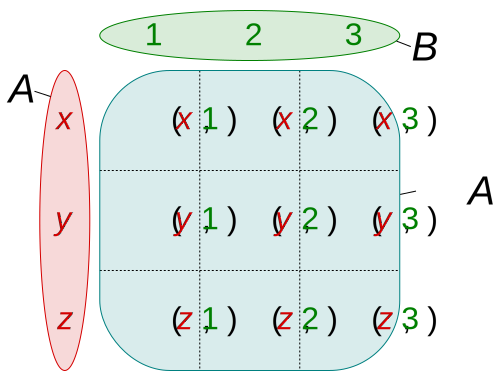
\includegraphics[width=0.3\linewidth]{010-pic.svg}	
% \end{center}  
 In the same sense, for sets $A_1, \ldots, A_n$
 the set of all \defi{$n$-tupels} is defined:
  	$$
 		A_1 \times \cdots \times
 		A_n
 		:=  \{ (a_1,\ldots, a_n) \mid a_1 \in A_1, \ldots, a_n \in A_n\}
 	$$
\end{Definition}
